\documentclass[11pt, titlepage]{article}

\usepackage[margin=1in]{geometry}
\usepackage[strict]{changepage}
\usepackage{float}
\usepackage{fancyhdr}
\usepackage{mhchem}
\usepackage{siunitx}
\usepackage{wrapfig, booktabs}
\usepackage{enumitem}
\usepackage{caption}
\usepackage{commath}
\usepackage{amsmath}
\usepackage[hang]{footmisc}
\usepackage{multicol}
\usepackage{amsfonts}
\usepackage{mathrsfs}
\usepackage{hyperref}
 \usepackage{graphicx}
 
\newcommand{\experimentDate}{1 May 2016}
\newcommand{\className}{STA 571}
\newcommand{\experimentNumber}{Final Project}
\author{Shijia Bian}
\newcommand{\authorLastName}{BIAN}
\title{Recommender System: Search Relevance Improvement}
\newcommand{\experimentShortName}{STA 571 Final Project}

\date{\parbox{\linewidth}{}}

\pagestyle{fancy}
\fancyhf{}
\rhead{\authorLastName\ \thepage}
\lhead{\experimentShortName}
\cfoot{\className\ -- \experimentNumber}

\usepackage{color}
\usepackage{sectsty}

\definecolor{WordSectionBlue}{RGB}{30, 90, 147}

\allsectionsfont{\color{WordSectionBlue}}

\newcommand{\gpmol}{\si{\gram\per\mol}}

\begin{document}
\maketitle
\setcounter{tocdepth}{1}
\section{Introduction}


The recommender system revolutionizes the way that people collect information and make decisions. As technology has weaved into the society and culture, the recommender system has a subtle influence on people's life. People gradually and unconsciously rely on the recommender system that can give them adequate suggestions based on personal historical data, or data from other users having the similar characteristics. The different recommender systems also compete for more sophisticated and efficient algorithms that can provide the users with more accurate recommending results. The growing participants in this technology century creates tremendous amount of user data for the recommender system to analyze. The size and the sparsity of the data challenges the algorithm on achieving well performed results. The collaborative filtering is one approach to handle the overloaded data set, and let the recommender system to provide customers with the recommendations based on the others' preferences [1]. This paper will implement the algorithm to improve the search relevance performance by adopting the methodology of the collaborative filtering. The solution is composed with feature engineering and Machine Learning algorithm. The experiment is studied upon the data generated from the searching engine of the Home Depot website.

\section{Related Work}


%What is the real-world problem your project will address? What data
%will motivate your methodology?  

There are different approaches the recommender system is adopting, such as the content-based recommendation, information retrieval, collaborative filtering and so on[2]. Different approaches are inclined to choose adequate algorithms according to their own methodologies and goals. 

\vspace{3mm} 
With the adoption of different approaches or combination of approaches, the recommender system is widely implemented to serve various purposes. The recommender system can be applied for product recommendation, such as Amazon.com and Pinterest. The Netflix Prize is a movie recommendation competition well known for adopting the collaborative filtering within this field. The Netflix Prize score matrix in Table 1 shows the scores the users give for movies. 'NaN' stands for the movie that the users haven't rated. Netflix is interested in predicting the score the user will give for the 'NaN', in terms of the history of this user and other users that have similar characteristics. Then, Netflix develops a new algorithm to recommend the right movies to the users. 

\vspace{3mm} 
Another application of the collaborative filtering is the searching engine system, such as Google and Bing. This application can be also adopted for the online ads competition. The list of results returned by the searching engine is ranked by relevance. The first result is expected to be the most pertinent to the users' needs. The potential web pages can be initially filtered out by the number of words match between the searching queries and the web pages. Then, the relevance score can be evaluated through textual and hyperlink relevance. The common technique is information retrieval[3]. 

\vspace{3mm} 
Therefore, the performance of the recommender system has a large impact on business. This final project will carry out an experiment of predicting relevance score. Feature engineering and machine learning algorithm together will be implemented to build up the algorithm. The relevance score measures the relevance between the searching query and a specific product. The data is provided by the "Home Depot Product Search Relevance" on  \href{<https://www.kaggle.com/c/home-depot-product-search-relevance>}{Kaggle}. 


\section{Problem definition} 

%Define this problem quantitatively. What question are you trying to
%solve? What are the random variables? What is the goal of the project?

\subsection{Motivation} 

\noindent
The customer searches for the products on Home Depot's website [4]. The customer expects Home Depot to give the expected result corresponding to the input queries. The customer experience can be elevated by improving the searching result accuracy. The search relevancy is defined to measure how matching between the searching queries and the returned result. Currently, human effort is spent on evaluating the relevance score. Home Depot wants to develop a new algorithm to automate this process and free the labor efforts.

\subsection{Dataset Overview} 


\noindent
There are four data sets provided by Home Depot: train.csv, product\_description.csv, attributes.csv, test.csv. 

\vspace{3mm} 
train.csv (Table 2) is the training set that has four informative columns. One column lists the searching term the user inputs into the searching engine. The other two columns list the product title and product ID of the corresponding returned product. The value type of product title is string. The fourth column is the relevance score rated by the labor effort. The relevance rating has three levels: irrelevant (1), partially relevant (2) and match (3). Three people will give the score together. The final score listed in this training data is the average of the three scores. The distribution of the relevance score from the training data is plotted in Figure 1. product\_description.csv (Table 3) has two columns: the product ID and the corresponding product description. The value of the product description is text. attributes.csv (Table 4) lists the attribute information for each product. Each of the product have multiple rows, and each row describes one attribute for that product. The test data is the same of as the train.csv, except that test.csv does not have the column of the relevance score. Our goal is to predict the relevance score for each product in the test.csv after training the model on the train.csv combined with the provided information.

\vspace{3mm} 
The row number of train.csv is 74,067. The row number of test.csv is 166,693. In the train data set, there are 54,667 unique products. In the test set, there are 97,460 unique products. Figure 2 shows that there are 27,699 unique products overlapping between the train data and the test data. The product listed in the product\_description.csv and attributes.csv have the information for all, except 16, unique products appearing in the train.csv and test.csv. Therefore, there is only 16 missing description or attribute information for the products in the training data and the test data. This amount of missing value is small enough to be ignored. Figure 3 shows that the number of words in each searching queries against the relevance score in the train data set. The lower relevance score tends to have shorter searching query. This makes sense that the shorter query cannot contain enough information and let the algorithm choose the most relevant results. 

\vspace{3mm} 
The primary goal of the project is to derive the features by using the given information, deliver the adequate machine learning algorithms and make prediction on the relevance scores for the test data set. 


\section{Models and Methods}

\subsection{Challenge}

Here are the three main difficulties of this project. These challenges should be carefully handled.

\begin{itemize}
\item Potential Overfitting Issue: Figure 2 illustrates that only $\frac{1}{3}$ products from the test data is shared by both the test and train data set. Around $\frac{2}{3}$ of the products in the test data are new, and $\frac{1}{2}$ of the train data is unique from the test data set. If the training model has overfitting issue, the bias will be enlarged in the test data set.
\item Model Sensitivity: the model should be able to distinguish and give the adequate relevance score for different queries that return the same products with different relevance scores. For example, the search queries "angle bracket" and "I bracket" both return the product "Simpson Strong-Tie 12-Gauge Angle". But the first query has relevance score 3, and the second query has relevance score 2.5. 
\item Word Matching and Tokenization: the word matching should have proper match disregard of the plural, tense and speech parts. For example, "table" should have a perfect match with "tables", same for "flexible" and "high of flexibility". In addition, the word has opposite meaning once adding a negative adjective. For example, the search item is looking for a "deep sink"; the word in the product description is "medium deep sink". Although there are words matching, but the meaning is opposite. 
\end{itemize}


\subsection{Feature Engineering}

The provided preliminary data cannot be used directly. They needs to be pre-processed before constructing the machine learning model and making predictions. All the work is carried in iPython Notebook.

\vspace{3mm} 
The attribute.csv should be aggregated by the product ID. In this way, one product ID is speaking to all the attributes in each row. The product description and this new attributes information should be left joint on the training data by product ID. Therefore, each of the product in the training data will have its product description and attributes information. One example of the row after left joint is shown in Table 5.

\vspace{3mm} 
Below is the list of final derived features from the product title, search term, product description and the attributes. These features can describe the relevance between the search item and the returned product. In other words, the features below can predict the relevance score. 
 
\begin{itemize}
\item the number of words in product description
\item the number of words in product title
\item the percentage of the words in search term match the product description
\item the percentage of the words in search term match the product title
\item the count of numbers in search item match the numbers in the the attribute 
\item the percentage of the count of numbers in search item match the numbers in the the attribute 
\item the number of words in search item
\item the count of numbers in the attribute
\end{itemize}


\subsection{Model}

Two models are chosen for the relevance score prediction: Random Forest (RF) and XGBoost. The validation criteria is root MSE: $RMSE = \sqrt{\frac{1}{n}\sum_{i=1}^n(y_i-\hat{y}_i)^2}$. The MSE in this paper means RMSE.

\vspace{3mm} 
The data was initially trained on the RF by using the first four features listed above. All the parameters in RF are set as default, except the number of estimator is 100. The test MSE is 0.74. With the same parameter setting, adding the fifth and sixth features above, the test MSE is reduced to 0.71.

\vspace{3mm} 
In the end of the model training, Random Forest (RF) and XGBoost are chosen together. The two models use all the eight derived features above. These two algorithms are all supervised learning, as we have both x values and y labels for our data. And the two methods are all tree-based methods. Both the algorithms are known for their accurate prediction and efficient speed. RF is very efficient at handling the large data set that has large features. RF is an average of the classification trees. The classification is given by the majority vote for that class. The internal out-of-bag error rate can help create an unbiased estimator, and de-correlate the correlations among the features through controling \texttt{mtry} (how deep each of the boosting tree should grow, if any features are highly correlated). RF can also provide a importance rank for the variables that is very convenient. The XGBoost is a gradient boosting algorithm, and it is based on the gradient boosting tree.  XGBoost is always considered as a alternative option for the random forest. XGBoost has advantage on speed over Random Forest. But XGBoost has to be tune more carefully than RF to avoid over-fitting. 

\vspace{3mm} 
In terms of the suggestions of using only the overlapping product to train the model, the test MSE is even worse by using either the two models ($75\%$). This might be due to the small amount of overlapping. Therefore, we only talks about using the entire train data for training the model in the next section.


\section{Results and validation}

\subsection{Random Forest}

The random forest model is tuned on two parameters: the number of estimators and the minimum number of leaf. The number of estimators controls the number of build-up trees for majority vote. The minimum number of leaf controls how deep each of the sampled tree should grow. The train MSE and the test MSE is listed in Table 6. As the parameter tuned with more iterations, the test MSE first decreases and then increases. The minimum test MSE reached is $0.62815$. 



\subsection{XGBoost}

Two objectives are chosen for XGBoost, \texttt{multi:softprob} and \texttt{reg:linear}. But the two objectives does not make a lot of difference in this problem. For the results below, I use \texttt{objective = 'reg:linear'}, due to the derived feature is intuitively linearly related to the relevence score. XGBoost is tuned on two parameters, the number of estimators and the learning rate. The result of the XGBoost MSE tunned on different parameters is listed in Table 7. The train MSE decreasing as the force of learning increases, but the test MSE increases once it reaches the minimum value.



\section{Conclusion}

XGBoost can achieve a lower train MSE than the RF does, but RF and XGBoost achieve similar test MSE with different tuned parameters. XGBoost requires more sophisticated skills in choosing the tuning parameter, and XGBoost also faces the higher risk of overfitting than the RF does, this is the reason why the test MSE of XGBoost is similar to that of RF, but the train MSE of XGBoost is much lower. By using the current derived features, the test MSE cannot be further improved. However, the test MSE can be further reduced, if more careful feature engineering techniques is carried on. Overall, the relevance score prediction for the searching engine system is a combination of feature engineering and Machine Learning algorithm. The business should further improve their recommender system by increasing the relevance score prediction, so that the returned products can have the right products appearing on the top of the list.
 

\section*{Supplementary Materials}

The proposal, poster, coding and written part will be uploaded to \href{<https://github.com/shijbian/STA571_Final_Project}{GitHub} repository shortly after the due date (11:55pm May 1, 2016).

\vspace{3mm} 
\noindent 
Due to the late script submission on Kaggle, the most updated test MSE won't appear on the Leadboard and \href{<https://www.kaggle.com/shijiabian}{my Kaggle} account. 

 
\newpage

\section*{Appendix: Table}


\begin{table}[H]
\centering
\label{my-label}
\begin{tabular}{|l|l|l|}
\hline
       & Movie A & Movie B \\ \hline
User A & 2       & NaN       \\ \hline
User B & NaN       & 3       \\ \hline
\end{tabular}
\caption{Netflix Prize Score Matrix}
\end{table}

\begin{table}[H]
\centering
\label{my-label}
\begin{tabular}{|l|l|l|l|l|}
\hline
id & product\_uid & product\_title                       & search\_term  & relevance \\ \hline
2  & 100001       & Simpson Strong-Tie,12-Gauge Angle    & angle bracket & 3         \\ \hline
3  & 100001       & Simpson Strong-Tie,12-Gauge Angle    & I bracket     & 2.5       \\ \hline
9  & 100002       & BEHR Premium,Textured DeckOver 1-gal & deck over     & 3         \\ \hline
\end{tabular}
\caption{train.csv}
\end{table}

\begin{table}[H]
\centering
\label{my-label}
\begin{tabular}{|l|l|}
\hline
product\_uid & product\_description                                                                                                                                                                                                                                                                 \\ \hline
100001       & \begin{tabular}[c]{@{}l@{}}Not only do angles,make joints stronger, they also provide more consistent, \\ straight corners.,Simpson Strong-Tie offers a wide variety of angles in various \\ sizes and,thicknesses to handle light-duty jobs or projects ...\end{tabular}            \\ \hline
100002       & \begin{tabular}[c]{@{}l@{}}BEHR Premium Textured,DECKOVER is an innovative solid color coating. \\ It will bring your old,,weathered wood or concrete back to life. The advanced \\ 100\% acrylic resin,formula creates a durable coating for your tired and worn ...\end{tabular}   \\ \hline
191872       & \begin{tabular}[c]{@{}l@{}}BEHR Premium Plus,Ultra Matte Interior Paint and Primer in One will change \\ the way you paint,and save you time. This performance-driven paint, featuring \\ NANOGUARD,technology, offers superior stain removal and excellent hide in ...\end{tabular} \\ \hline
\end{tabular}
\caption{product\_description.csv}
\end{table}

\begin{table}[H]
\centering
\begin{tabular}{|l|l|l|}
\hline
product\_uid & name     & value                                                                     \\ \hline
100001       & Bullet01 & Versatile connector,for various 90å¡ connections and home repair projects \\ \hline
100001       & Bullet02 & Stronger than,angled nailing or screw fastening alone                     \\ \hline
100001       & Bullet03 & Help ensure joints,are consistently straight and strong                   \\ \hline
100001       & Bullet04 & Dimensions: 3 in. x,3 in. x 1-1/2 in.                                     \\ \hline
100001       & Bullet05 & Made from 12-Gauge,steel                                                  \\ \hline
100001       & Bullet06 & Galvanized for,extra corrosion resistance                                 \\ \hline
100001       & Bullet07 & Install with 10d,common nails or,9 x 1-1/2 in.,Strong-Drive SD screws     \\ \hline
\end{tabular}
\label{attributes.csv}
\caption{attributes.csv}
\end{table}

\begin{table}[H]
\centering
\label{my-label}
\begin{tabular}{|l|l|l|l|l|l|l|}
\hline
id & product\_uid & product\_title                    & search\_term  & relevance & product\_description                                                                                     & attributes                                                                                             \\ \hline
2  & 100001       & Simpson... & angle bracket... & 3         & \begin{tabular}[c]{@{}l@{}}Not only do angles,\\ make joints stronger, \\ they also provide...\end{tabular} & \begin{tabular}[c]{@{}l@{}}Bullet01: Versatile \\ connector,for various \\ 90 connections...\end{tabular} \\ \hline
\end{tabular}
\caption{The Joint Table with All the Features for Each Product}
\end{table}


\begin{table}[H]
\centering
\label{my-label}
\begin{tabular}{|c|c|c|c|}
\hline
n estimator & min sample leaf & train MSE & test MSE \\ \hline
5           & 5               & 0.54252   & 0.63936  \\ \hline
10          & 10              & 0.54322   & 0.6298   \\ \hline
50          & 50              & 0.61378   & 0.62815  \\ \hline
100         & 100             & 0.62310   & 0.63362  \\ \hline
150         & 150             & 0.62765   & 0.63702  \\ \hline
200         & 200             & 0.63074   & 0.63826  \\ \hline
200         & 5               & 0.51000   & 0.62846  \\ \hline
300         & 5               & 0.50981   & 0.62785  \\ \hline
\end{tabular}
\caption{Random Forest MSE}
\end{table}


\begin{table}[H]
\centering
\label{my-label}
\begin{tabular}{|c|c|c|c|c|}
\hline
max\_depth & n\_estimators & learning\_rate & train MSE & test MSE \\ \hline
3          & 5             & 0.01           & 0.60163   & 0.60607  \\ \hline
5          & 10            & 0.01           & 0.62268   & 0.63074  \\ \hline
7          & 50            & 0.01           & 0.6038    & 0.61854  \\ \hline
9          & 100           & 0.15           & 0.55392   & 0.62837  \\ \hline
9          & 1000          & 0.15           & 0.3101    & 0.64705  \\ \hline
\end{tabular}
\caption{XGBoost MSE}
\end{table}

\section*{Appendix: Figure}

\begin{figure}[H]
  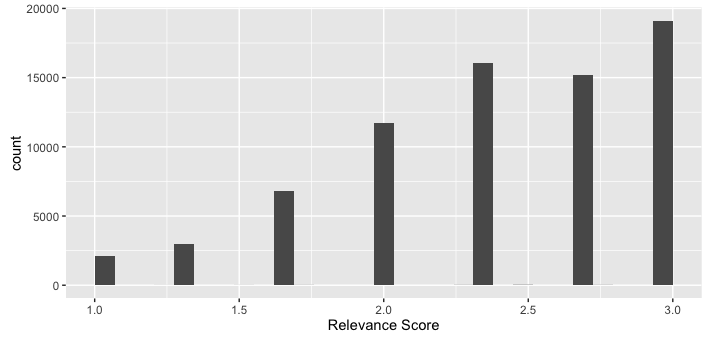
\includegraphics[width=\linewidth]{relevance_score.png}
  \caption{Histogram of the Relevance Score in Training Data}
  \label{fig:boat1}
\end{figure}

\begin{figure}[H]
  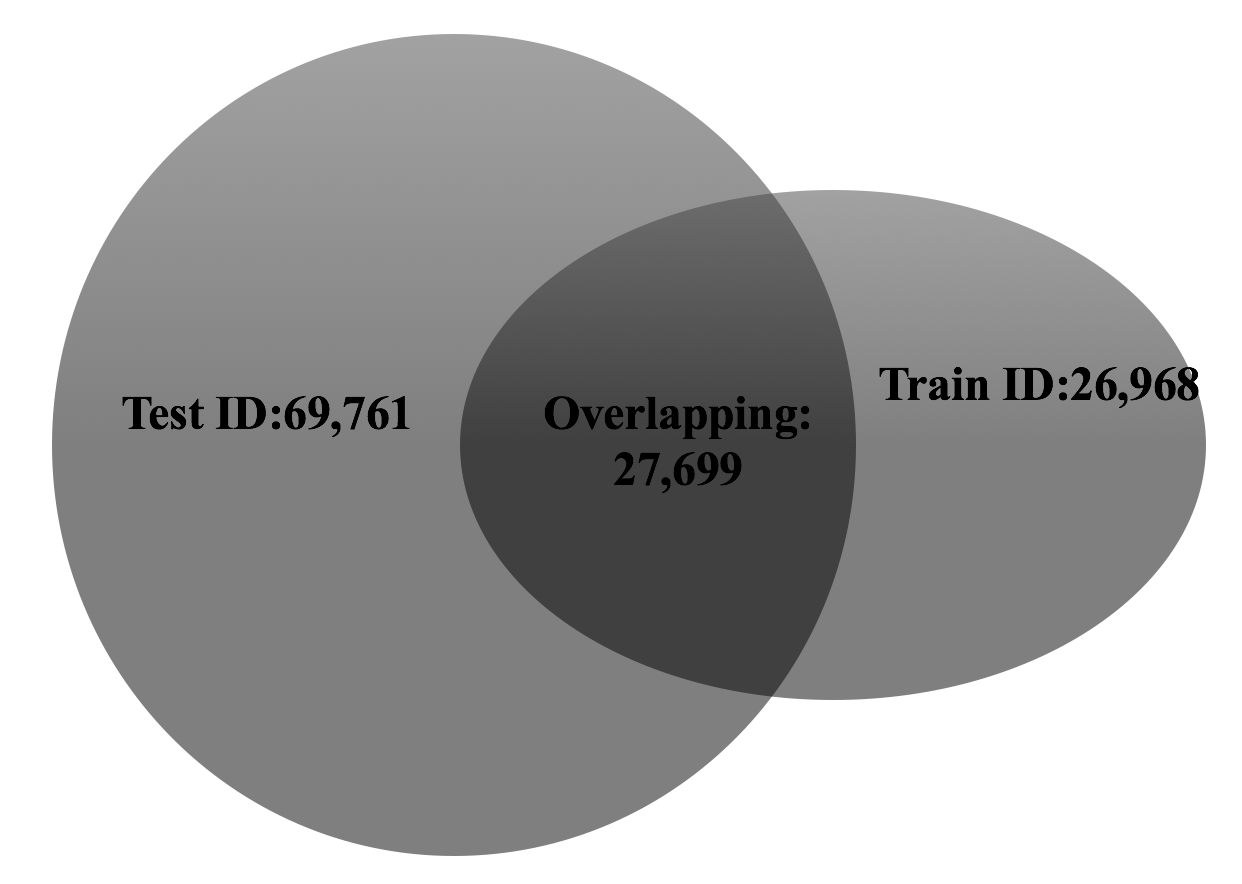
\includegraphics[scale=0.7]{train_test_data.png}
  \caption{The Unique Product Visualization in Train and Test Data [6]}
  \label{fig:boat1}
\end{figure}

\begin{figure}[H]
  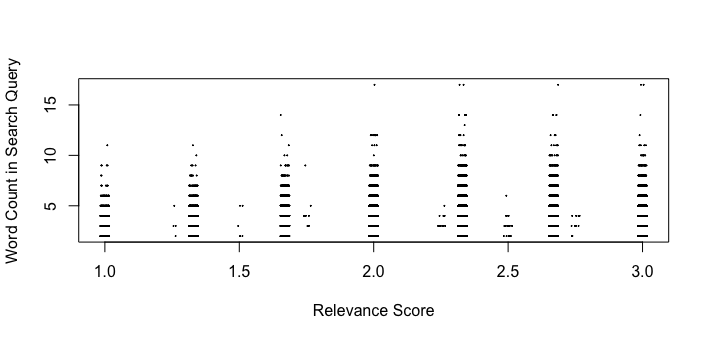
\includegraphics[width=\linewidth]{query_count.png}
  \caption{The Number of Word in the Searching Query Against the Replevance Score}
  \label{fig:boat1}
\end{figure}


\section*{Reference}
[1] Ekstrand, Michael D., John Riedl, and Joseph Konstan.\textit{ Collaborative Filtering Recommender Systems}. Hanover, MA: Now, 2011. Print.

\noindent 
[2] (Kberberi@mpi-Inf.mpg.de), Berberich, Klaus, Gupta, Dhruv. \textit{Advanced Topics in Information Retrieval-Recommender Systems}. Saarland University, WS 2014/2015. Web.

\noindent 
[3] Hugo Zaragoza, Marc Najork. \textit{Web Search Relevance Ranking}. Yahoo! Research, Barcelona, Spain. Microsoft Research, Mountain View, CA.

\noindent 
[4] Home Depot Product Search Relevance. \textit{Predict the relevance of search results on homedepot.com}. Home Depot. \href{<https://www.kaggle.com/c/home-depot-product-search-relevance>}{Kaggle}. 


\noindent 
[5] Greg Linden , Brent Smith , Jeremy York, \textit{Amazon.com Recommendations: Item-to-Item Collaborative Filtering}, IEEE Internet Computing, v.7 n.1, p.76-80, January 2003  [doi>10.1109/MIC.2003.1167344]

\noindent 
[6] Brian Carter. \textit{HomeDepot First Data Exploration}. Home Depot Product Search Relevance. \href{<https://www.kaggle.com/briantc/home-depot-product-search-relevance/homedepot-first-dataexploreation-k>}{Kaggle.com}, 19 February 2016. Web.


\end{document}